% METADATA SUBSTRATE DESIGN VISUALS — ADDENDUM (A1–A6)
% Companion to METADATA_CACHE_DRIFT_REVIEW_ADDENDUM.md; same visual language as v2.
% Compile: pdflatex METADATA_DESIGN_VISUALS_ADDENDUM.tex (twice)
\documentclass[10pt]{article}
\usepackage[a4paper,landscape,margin=9mm]{geometry}
\usepackage[utf8]{inputenc}
\usepackage[T1]{fontenc}
\usepackage[sc]{mathpazo}
\usepackage{microtype}
\usepackage{tikz}
\usetikzlibrary{arrows.meta,positioning,fit,calc,backgrounds,shapes.geometric,shapes.multipart,matrix}
\usepackage{xcolor}
\usepackage{colortbl}
\usepackage{array,tabularx,booktabs}
\usepackage{adjustbox}
\usepackage{hyperref}
\hypersetup{hidelinks}
\pagestyle{empty}
\setlength{\parindent}{0pt}
\setlength{\tabcolsep}{4pt}
\renewcommand{\arraystretch}{1.16}

% Palette: identical to v2.
\definecolor{store}{HTML}{EAF0FF}
\definecolor{snap}{HTML}{EAF8EC}
\definecolor{engine}{HTML}{FFF3E4}
\definecolor{session}{HTML}{FFF0EE}
\definecolor{gate}{HTML}{E8F7F5}
\definecolor{obs}{HTML}{F6EDFA}
\definecolor{future}{HTML}{FFF9D9}
\definecolor{risk}{HTML}{FFE3E3}
\definecolor{good}{HTML}{E2F5E7}
\definecolor{external}{HTML}{F5F5F5}
\definecolor{ink}{HTML}{263238}
\definecolor{muted}{HTML}{607D8B}
\definecolor{green}{HTML}{39784A}
\definecolor{orange}{HTML}{B56A24}
\definecolor{red}{HTML}{B54A4A}
\definecolor{blue}{HTML}{3F6FB5}
\definecolor{purple}{HTML}{7A4E9B}

\newcommand{\code}[1]{\texttt{\detokenize{#1}}}

\tikzset{
  >=Latex,
  every node/.style={font=\small,text=ink},
  box/.style={draw=ink!55,rounded corners=2.5pt,fill=store,align=center,inner sep=4pt,minimum height=10mm},
  snapbox/.style={box,fill=snap,draw=green!65},
  enginebox/.style={box,fill=engine,draw=orange!70},
  sessbox/.style={box,fill=session,draw=red!65},
  gatebox/.style={box,fill=gate,draw=green!70},
  obsbox/.style={box,fill=obs,draw=purple!65},
  futurebox/.style={box,fill=future,draw=orange!80},
  riskbox/.style={box,fill=risk,draw=red!75},
  goodbox/.style={box,fill=good,draw=green!75},
  extbox/.style={box,fill=external,draw=ink!45,dashed},
  state/.style={draw=ink!60,rounded corners=7pt,fill=store,minimum width=29mm,minimum height=10mm,align=center,inner sep=3pt},
  arrow/.style={->,very thick,draw=ink!75},
  thinarr/.style={->,thick,draw=ink!65},
  dashedarr/.style={->,thick,dashed,draw=purple!80},
  hot/.style={->,very thick,draw=red!80},
  failarr/.style={->,thick,dashed,draw=red!75},
  note/.style={draw=ink!25,rounded corners=2pt,fill=white,align=left,inner sep=5pt,font=\footnotesize,text width=62mm},
  smallnote/.style={draw=ink!25,rounded corners=2pt,fill=white,align=left,inner sep=4pt,font=\scriptsize,text width=42mm},
  pill/.style={draw=ink!35,rounded corners=7pt,fill=white,inner xsep=5pt,inner ysep=2pt,font=\footnotesize\bfseries},
  caption/.style={font=\scriptsize,align=center,fill=white,inner sep=1.3pt},
  life/.style={draw=ink!35,thick},
  msg/.style={->,thick,draw=ink!75,font=\scriptsize},
  msgd/.style={->,thick,dashed,draw=purple!80,font=\scriptsize},
  head/.style={box,minimum width=30mm,minimum height=8mm,font=\footnotesize\bfseries},
}

\newcommand{\pagehead}[2]{%
  \begin{minipage}[t]{0.70\linewidth}
    {\Large\bfseries #1}\\[-1mm]
    {\small\color{muted}#2}
  \end{minipage}\hfill
  \begin{minipage}[t]{0.28\linewidth}\raggedleft
    {\footnotesize Metadata substrate - review visuals v2 \textbf{addendum}}\\
    {\scriptsize companion to REVIEW\_ADDENDUM.md - 2026-07-06}
  \end{minipage}
  \vspace{2.5mm}\hrule\vspace{3.5mm}
}

\newcommand{\legend}{%
\tikz[baseline=-0.7ex]\node[box,minimum width=7mm,minimum height=4mm,inner sep=1pt]{}; store/registry\quad
\tikz[baseline=-0.7ex]\node[snapbox,minimum width=7mm,minimum height=4mm,inner sep=1pt]{}; pure snapshot\quad
\tikz[baseline=-0.7ex]\node[enginebox,minimum width=7mm,minimum height=4mm,inner sep=1pt]{}; engine/hydration\quad
\tikz[baseline=-0.7ex]\node[sessbox,minimum width=7mm,minimum height=4mm,inner sep=1pt]{}; sessions/data plane\quad
\tikz[baseline=-0.7ex]\node[gatebox,minimum width=7mm,minimum height=4mm,inner sep=1pt]{}; contract/privacy gate\quad
\tikz[baseline=-0.7ex]\node[futurebox,minimum width=7mm,minimum height=4mm,inner sep=1pt]{}; proposed cache\quad
\tikz[baseline=-0.7ex]\node[riskbox,minimum width=7mm,minimum height=4mm,inner sep=1pt]{}; correction/hazard\quad
\tikz[baseline=-0.7ex]\node[obsbox,minimum width=7mm,minimum height=4mm,inner sep=1pt]{}; observability
}

% coverage dots for page A4
\newcommand{\hit}{\tikz[baseline=-0.6ex]\fill[green] (0,0) circle (1.5mm);}
\newcommand{\hint}{\tikz[baseline=-0.6ex]{\draw[orange,thick] (0,0) circle (1.5mm);\fill[orange] (0,0) -- (90:1.5mm) arc (90:270:1.5mm) -- cycle;}}
\newcommand{\miss}{\tikz[baseline=-0.6ex]\draw[red,thick] (0,0) circle (1.5mm);}
\newcommand{\na}{\textcolor{muted}{--}}

\begin{document}

% =====================================================================
% A1. ensureFresh DECISION PROCEDURE
% =====================================================================
\pagehead{A1. \code{ensureFresh(policy)} - the decision procedure}
{Addendum \S4.2 as a flowchart. Waits are races: a timeout stops waiting, it never cancels the shared lane work. Implement this page 1:1.}
\legend\par\vspace{4mm}

\begin{adjustbox}{max width=\linewidth,max height=0.82\textheight,center}
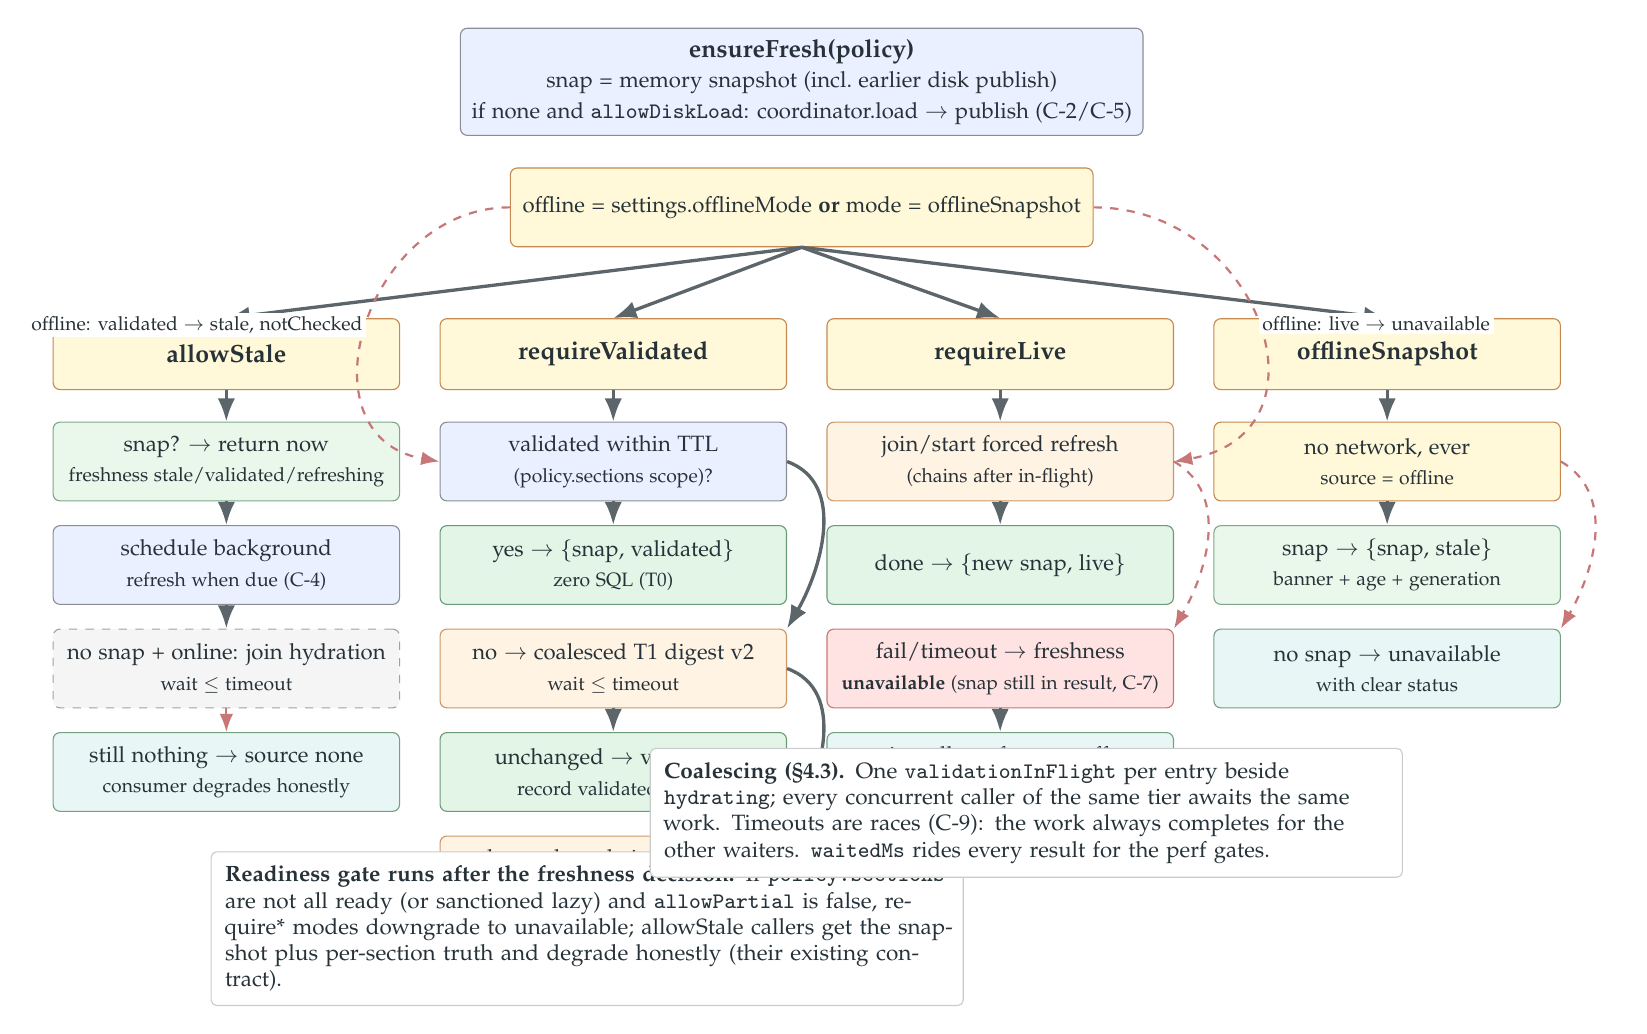
\begin{tikzpicture}[node distance=5mm and 6mm]

\node[box,minimum width=74mm] (entry) {\textbf{ensureFresh(policy)}\\\footnotesize snap = memory snapshot (incl.\ earlier disk publish)\\\footnotesize if none and \code{allowDiskLoad}: coordinator.load $\to$ publish (C-2/C-5)};
\node[futurebox,minimum width=74mm,below=4mm of entry] (offline) {\footnotesize offline = settings.offlineMode \textbf{or} mode = offlineSnapshot};

% four mode columns
\node[futurebox,minimum width=44mm,minimum height=9mm,below left=9mm and 51mm of offline.south] (m1) {\textbf{allowStale}};
\node[futurebox,minimum width=44mm,minimum height=9mm,right=5mm of m1] (m2) {\textbf{requireValidated}};
\node[futurebox,minimum width=44mm,minimum height=9mm,right=5mm of m2] (m3) {\textbf{requireLive}};
\node[futurebox,minimum width=44mm,minimum height=9mm,right=5mm of m3] (m4) {\textbf{offlineSnapshot}};
\foreach \m in {m1,m2,m3,m4} {\draw[arrow] (offline.south) -- (\m.north);}

% allowStale column
\node[snapbox,minimum width=44mm,below=4mm of m1] (a1) {\footnotesize snap? $\to$ return now\\\scriptsize freshness stale/validated/refreshing};
\node[box,minimum width=44mm,below=3mm of a1] (a2) {\footnotesize schedule background\\\scriptsize refresh when due (C-4)};
\node[extbox,minimum width=44mm,below=3mm of a2] (a3) {\footnotesize no snap + online: join hydration\\\scriptsize wait $\le$ timeout};
\node[gatebox,minimum width=44mm,below=3mm of a3] (a4) {\footnotesize still nothing $\to$ source none\\\scriptsize consumer degrades honestly};
\draw[arrow] (m1) -- (a1);\draw[arrow] (a1) -- (a2);\draw[arrow] (a2) -- (a3);\draw[failarr] (a3) -- (a4);

% requireValidated column
\node[box,minimum width=44mm,below=4mm of m2] (b1) {\footnotesize validated within TTL\\\scriptsize (policy.sections scope)?};
\node[goodbox,minimum width=44mm,below=3mm of b1] (b2) {\footnotesize yes $\to$ \{snap, validated\}\\\scriptsize zero SQL (T0)};
\node[enginebox,minimum width=44mm,below=3mm of b2] (b3) {\footnotesize no $\to$ coalesced T1 digest v2\\\scriptsize wait $\le$ timeout};
\node[goodbox,minimum width=44mm,below=3mm of b3] (b4) {\footnotesize unchanged $\to$ validated\\\scriptsize record validatedAtUtc};
\node[enginebox,minimum width=44mm,below=3mm of b4] (b5) {\footnotesize changed $\to$ chained refresh\\\scriptsize done: live -- timeout: stale+refreshing};
\draw[arrow] (m2) -- (b1);\draw[arrow] (b1) -- (b2);\draw[arrow] (b1.east) to[out=-20,in=60] (b3.north east);\draw[arrow] (b3) -- (b4);\draw[arrow] (b3.east) to[out=-20,in=60] (b5.north east);

% requireLive column
\node[enginebox,minimum width=44mm,below=4mm of m3] (c1) {\footnotesize join/start forced refresh\\\scriptsize (chains after in-flight)};
\node[goodbox,minimum width=44mm,below=3mm of c1] (c2) {\footnotesize done $\to$ \{new snap, live\}};
\node[riskbox,minimum width=44mm,below=3mm of c2] (c3) {\footnotesize fail/timeout $\to$ freshness\\\scriptsize \textbf{unavailable} (snap still in result, C-7)};
\node[gatebox,minimum width=44mm,below=3mm of c3] (c4) {\footnotesize strict caller refuses or offers\\\scriptsize explicit offlineSnapshot path};
\draw[arrow] (m3) -- (c1);\draw[arrow] (c1) -- (c2);\draw[failarr] (c1.east) to[out=-30,in=60] (c3.north east);\draw[arrow] (c3) -- (c4);

% offlineSnapshot column
\node[futurebox,minimum width=44mm,below=4mm of m4] (d1) {\footnotesize no network, ever\\\scriptsize source = offline};
\node[snapbox,minimum width=44mm,below=3mm of d1] (d2) {\footnotesize snap $\to$ \{snap, stale\}\\\scriptsize banner + age + generation};
\node[gatebox,minimum width=44mm,below=3mm of d2] (d3) {\footnotesize no snap $\to$ unavailable\\\scriptsize with clear status};
\draw[arrow] (m4) -- (d1);\draw[arrow] (d1) -- (d2);\draw[failarr] (d1.east) to[out=-30,in=60] (d3.north east);

% offline shortcuts into strict lanes
\draw[failarr] (offline.west) to[out=180,in=170,looseness=1.4] node[caption,left]{offline: validated $\to$ stale, notChecked} (b1.west);
\draw[failarr] (offline.east) to[out=0,in=10,looseness=1.6] node[caption,right]{offline: live $\to$ unavailable} (c1.east);

\node[note,below=5mm of a4,text width=92mm,anchor=north west,xshift=-2mm] (n1) {\textbf{Readiness gate runs after the freshness decision.} If \code{policy.sections} are not all ready (or sanctioned lazy) and \code{allowPartial} is false, require* modes downgrade to unavailable; allowStale callers get the snapshot plus per-section truth and degrade honestly (their existing contract).};
\node[note,below=5mm of d3,text width=92mm,anchor=north east,xshift=2mm] (n2) {\textbf{Coalescing (\S4.3).} One \code{validationInFlight} per entry beside \code{hydrating}; every concurrent caller of the same tier awaits the same work. Timeouts are races (C-9): the work always completes for the other waiters. \code{waitedMs} rides every result for the perf gates.};

\end{tikzpicture}
\end{adjustbox}

\newpage

% =====================================================================
% A2. DISK PROTOCOL + TORN-WRITE MATRIX
% =====================================================================
\pagehead{A2. Disk protocol: atomic writes, torn-write recovery, two windows}
{Every readable state is old-valid or new-valid by construction. The reader trusts nothing the manifest's SHA does not vouch for.}
\legend\par\vspace{4mm}

\begin{adjustbox}{max width=\linewidth,max height=0.82\textheight,center}
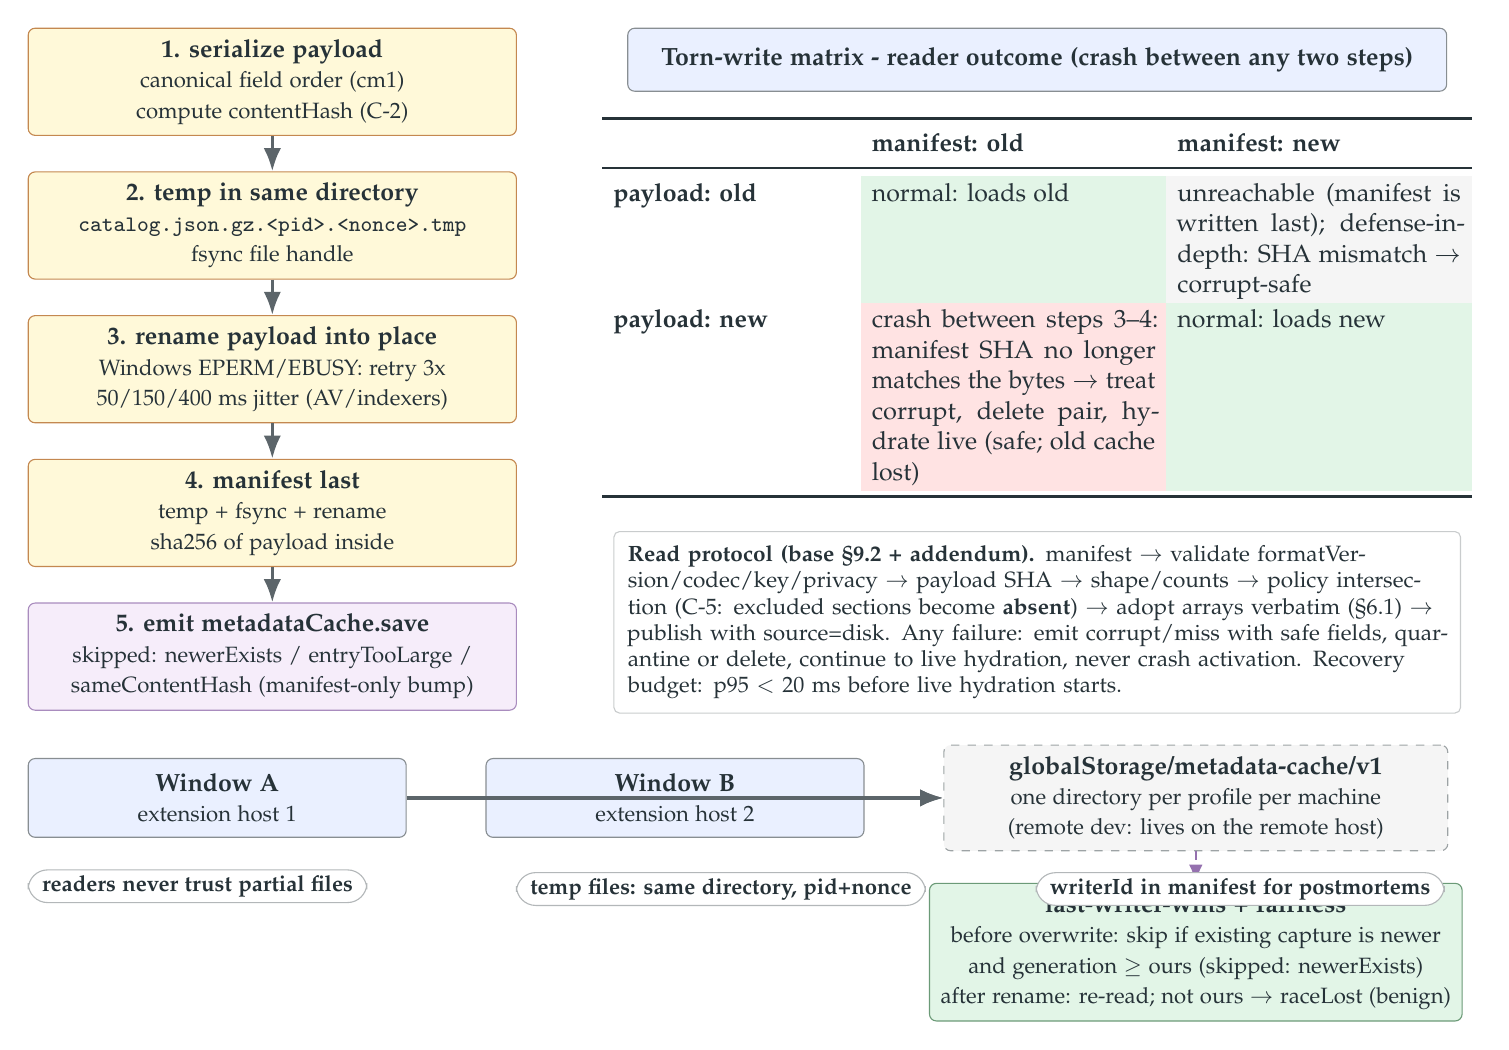
\begin{tikzpicture}[node distance=4.5mm and 8mm]

% write column
\node[futurebox,minimum width=62mm] (w1) {\textbf{1. serialize payload}\\\footnotesize canonical field order (cm1)\\\footnotesize compute contentHash (C-2)};
\node[futurebox,minimum width=62mm,below=of w1] (w2) {\textbf{2. temp in same directory}\\\footnotesize \code{catalog.json.gz.<pid>.<nonce>.tmp}\\\footnotesize fsync file handle};
\node[futurebox,minimum width=62mm,below=of w2] (w3) {\textbf{3. rename payload into place}\\\footnotesize Windows EPERM/EBUSY: retry 3x\\\footnotesize 50/150/400 ms jitter (AV/indexers)};
\node[futurebox,minimum width=62mm,below=of w3] (w4) {\textbf{4. manifest last}\\\footnotesize temp + fsync + rename\\\footnotesize sha256 of payload inside};
\node[obsbox,minimum width=62mm,below=of w4] (w5) {\textbf{5. emit metadataCache.save}\\\footnotesize skipped: newerExists / entryTooLarge /\\\footnotesize sameContentHash (manifest-only bump)};
\draw[arrow] (w1)--(w2);\draw[arrow] (w2)--(w3);\draw[arrow] (w3)--(w4);\draw[arrow] (w4)--(w5);

% torn matrix
\node[box,minimum width=104mm,minimum height=8mm,right=14mm of w1.north east,anchor=north west] (mt) {\textbf{Torn-write matrix - reader outcome (crash between any two steps)}};
\node[below=2mm of mt.south,anchor=north,xshift=0mm] (tbl) {%
\begin{tabular}{p{30mm}p{36mm}p{36mm}}
\toprule
 & \textbf{manifest: old} & \textbf{manifest: new} \\
\midrule
\textbf{payload: old} & \cellcolor{good} normal: loads old & \cellcolor{external} unreachable (manifest is written last); defense-in-depth: SHA mismatch $\to$ corrupt-safe \\[1mm]
\textbf{payload: new} & \cellcolor{risk} crash between steps 3--4: manifest SHA no longer matches the bytes $\to$ treat corrupt, delete pair, hydrate live (safe; old cache lost) & \cellcolor{good} normal: loads new \\
\bottomrule
\end{tabular}};

\node[note,below=3mm of tbl.south,anchor=north,text width=104mm] (rd) {\textbf{Read protocol (base \S9.2 + addendum).} manifest $\to$ validate formatVersion/codec/key/privacy $\to$ payload SHA $\to$ shape/counts $\to$ policy intersection (C-5: excluded sections become \textbf{absent}) $\to$ adopt arrays verbatim (\S6.1) $\to$ publish with source=disk. Any failure: emit corrupt/miss with safe fields, quarantine or delete, continue to live hydration, never crash activation. Recovery budget: p95 $<$ 20 ms before live hydration starts.};

% two windows
\node[box,minimum width=48mm,below=6mm of w5.south west,anchor=north west] (win1) {\textbf{Window A}\\\footnotesize extension host 1};
\node[box,minimum width=48mm,right=10mm of win1] (win2) {\textbf{Window B}\\\footnotesize extension host 2};
\node[extbox,minimum width=64mm,right=10mm of win2] (gs) {\textbf{globalStorage/metadata-cache/v1}\\\footnotesize one directory per profile per machine\\\footnotesize (remote dev: lives on the remote host)};
\draw[arrow] (win1.east) to[out=0,in=180] (gs.west);
\draw[arrow] (win2.east) -- (gs.west);
\node[goodbox,minimum width=64mm,below=4mm of gs] (lww) {\textbf{last-writer-wins + fairness}\\\footnotesize before overwrite: skip if existing capture is newer\\\footnotesize and generation $\ge$ ours (skipped: newerExists)\\\footnotesize after rename: re-read; not ours $\to$ raceLost (benign)};
\draw[dashedarr] (gs) -- (lww);

\node[pill,below=4mm of win1.south west,anchor=north west] {readers never trust partial files};
\node[pill,right=4mm of {$(win1.south west)+(58mm,-6.5mm)$}] {temp files: same directory, pid+nonce};
\node[pill,right=4mm of {$(win1.south west)+(124mm,-6.5mm)$}] {writerId in manifest for postmortems};

\end{tikzpicture}
\end{adjustbox}

\newpage

% =====================================================================
% A3. READINESS x FRESHNESS - THE TWO-AXIS HONESTY MAP
% =====================================================================
\pagehead{A3. Readiness $\times$ freshness: the two-axis honesty map}
{Corrections C-3/C-5/C-6/C-7 on one page. Readiness answers ``is this section trustworthy in this snapshot''; freshness answers ``is this snapshot recent enough for this caller''. Never collapse them.}
\legend\par\vspace{4mm}

\begin{adjustbox}{max width=\linewidth,max height=0.82\textheight,center}
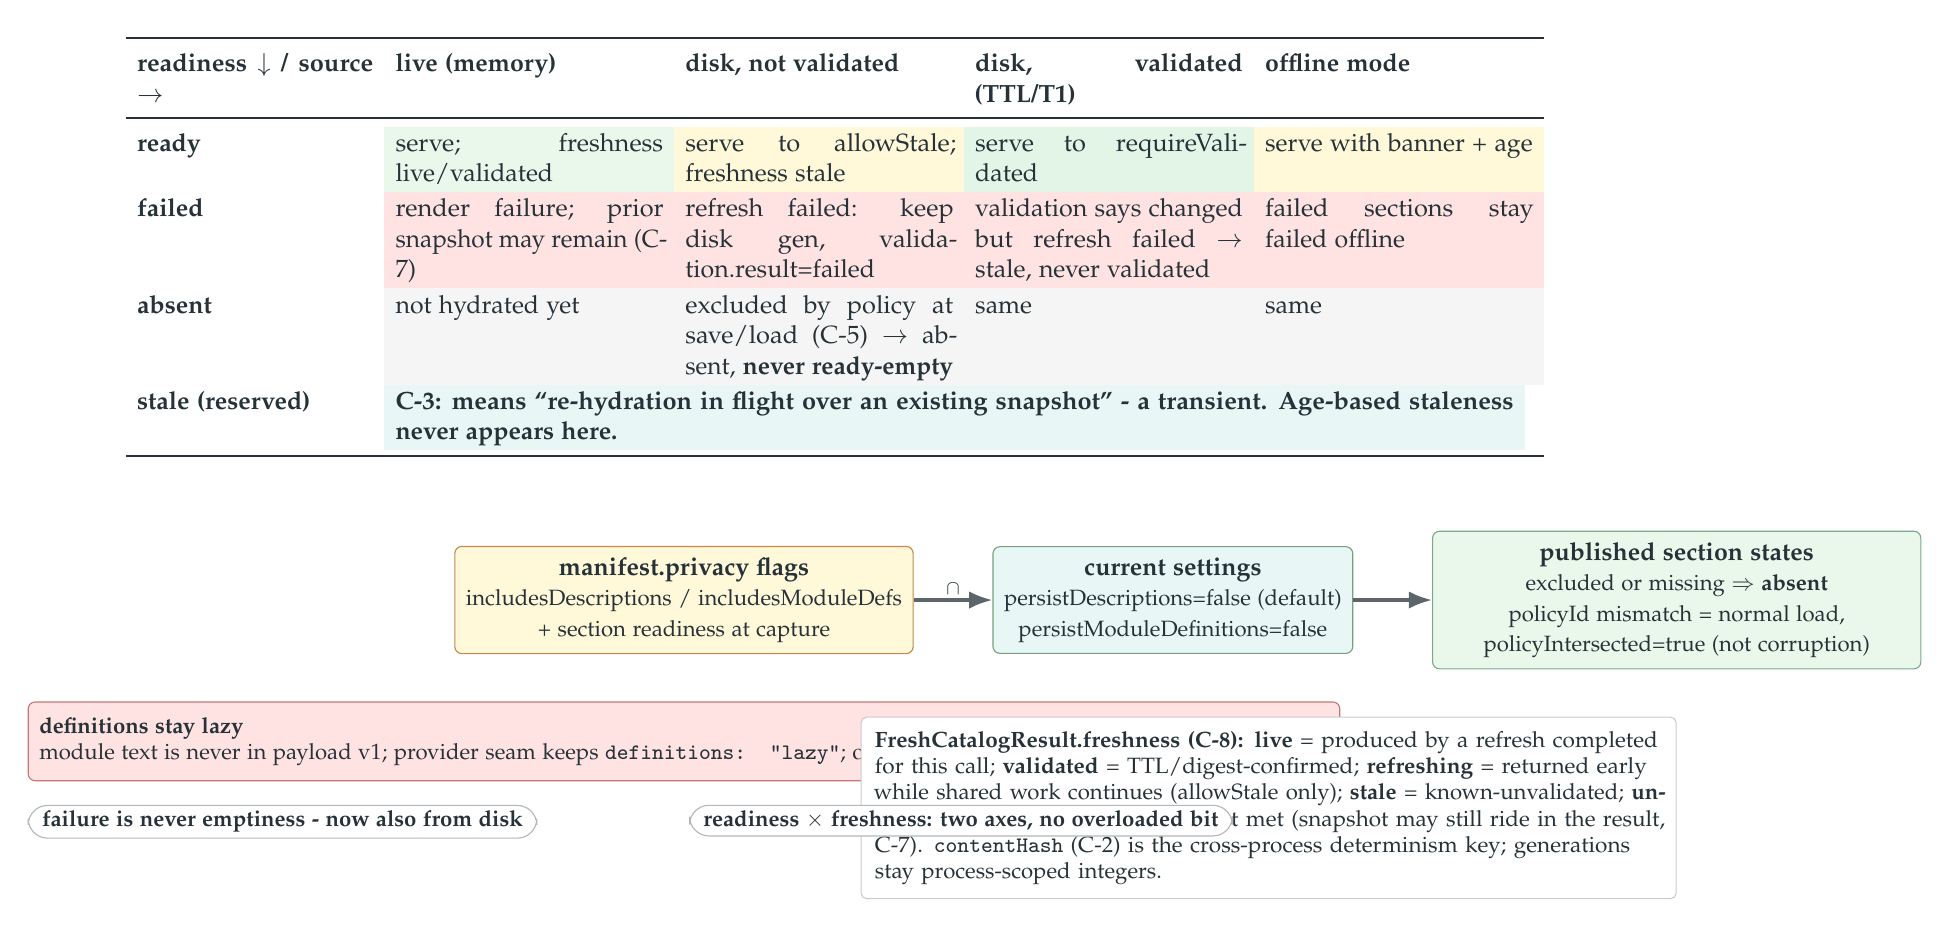
\begin{tikzpicture}[node distance=5mm and 8mm]

\node (grid) {%
\begin{tabular}{p{30mm}p{34mm}p{34mm}p{34mm}p{34mm}}
\toprule
\textbf{readiness $\downarrow$ / source $\rightarrow$} & \textbf{live (memory)} & \textbf{disk, not validated} & \textbf{disk, validated (TTL/T1)} & \textbf{offline mode} \\
\midrule
\textbf{ready} & \cellcolor{snap} serve; freshness live/validated & \cellcolor{future} serve to allowStale; freshness stale & \cellcolor{good} serve to requireValidated & \cellcolor{future} serve with banner + age \\[1mm]
\textbf{failed} & \cellcolor{risk} render failure; prior snapshot may remain (C-7) & \cellcolor{risk} refresh failed: keep disk gen, validation.result=failed & \cellcolor{risk} validation says changed but refresh failed $\to$ stale, never validated & \cellcolor{risk} failed sections stay failed offline \\[1mm]
\textbf{absent} & \cellcolor{external} not hydrated yet & \cellcolor{external} excluded by policy at save/load (C-5) $\to$ absent, \textbf{never ready-empty} & \cellcolor{external} same & \cellcolor{external} same \\[1mm]
\textbf{stale (reserved)} & \multicolumn{4}{>{\cellcolor{gate}}p{142mm}}{\textbf{C-3: means ``re-hydration in flight over an existing snapshot'' - a transient. Age-based staleness never appears here.}} \\
\bottomrule
\end{tabular}};

% intersection mini-diagram
\node[futurebox,minimum width=56mm,below left=10mm and -10mm of grid.south] (man) {\textbf{manifest.privacy flags}\\\footnotesize includesDescriptions / includesModuleDefs\\\footnotesize + section readiness at capture};
\node[gatebox,minimum width=44mm,right=10mm of man] (cur) {\textbf{current settings}\\\footnotesize persistDescriptions=false (default)\\\footnotesize persistModuleDefinitions=false};
\node[snapbox,minimum width=62mm,right=10mm of cur] (out) {\textbf{published section states}\\\footnotesize excluded or missing $\Rightarrow$ \textbf{absent}\\\footnotesize policyId mismatch = normal load,\\\footnotesize policyIntersected=true (not corruption)};
\draw[arrow] (man.east) -- node[caption,above]{$\cap$} (cur.west);
\draw[arrow] (cur.east) -- (out.west);

\node[riskbox,minimum width=58mm,below=6mm of man,align=left,font=\footnotesize] (defs) {\textbf{definitions stay lazy}\\ module text is never in payload v1; provider seam keeps \code{definitions: "lazy"}; offline getDefinition = honest refusal, not empty};
\node[note,below=6mm of out,text width=100mm,anchor=north east,xshift=0mm] (fr) {\textbf{FreshCatalogResult.freshness (C-8):} \textbf{live} = produced by a refresh completed for this call; \textbf{validated} = TTL/digest-confirmed; \textbf{refreshing} = returned early while shared work continues (allowStale only); \textbf{stale} = known-unvalidated; \textbf{unavailable} = the policy's bar was not met (snapshot may still ride in the result, C-7). \code{contentHash} (C-2) is the cross-process determinism key; generations stay process-scoped integers.};

\node[pill,below=3mm of defs.south west,anchor=north west] {failure is never emptiness - now also from disk};
\node[pill,right=6mm of {$(defs.south west)+(78mm,-5mm)$}] {readiness $\times$ freshness: two axes, no overloaded bit};

\end{tikzpicture}
\end{adjustbox}

\newpage

% =====================================================================
% A4. DRIFT DETECTOR COVERAGE MATRIX
% =====================================================================
\pagehead{A4. Drift detector coverage - what each trigger can and cannot see}
{H-1/H-5 on one page. Fill the live column of truth from the \code{metadata-drift.matrix.live} scenario, not from prose. The sp\_rename-from-elsewhere cell is why digest v2 exists.}
\legend\par\vspace{4mm}

\begin{center}
\hit\ detects\qquad \hint\ heuristic / partial\qquad \miss\ blind\qquad \na\ not applicable
\end{center}
\vspace{2mm}

\begin{adjustbox}{max width=\linewidth,max height=0.62\textheight,center}
\begin{tabular}{p{52mm}cccccc}
\toprule
\textbf{change class} & \textbf{A sniff (local)} & \textbf{B digest v1} & \textbf{B digest v2} & \textbf{TTL (T0)} & \textbf{T2 section (future)} & \textbf{C explicit} \\
\midrule
CREATE/DROP object - in this editor & \hit & \hit & \hit & \na & \hit & \hit \\
CREATE/DROP object - external client & \miss & \hit & \hit & \na & \hit & \hit \\
ALTER object (modify\_date bumps) - external & \miss & \hit & \hit & \na & \hit & \hit \\
\rowcolor{risk} sp\_rename - external client & \miss & \textbf{\miss} & \hit & \na & \hit & \hit \\
sp\_rename - in this editor & \hit & \miss & \hit & \na & \hit & \hit \\
\rowcolor{risk} ALTER SCHEMA \ldots TRANSFER - external & \miss & \textbf{\miss} & \hit & \na & \hit & \hit \\
Column/key/FK/param drift w/o modify\_date bump & \miss & \miss & \miss & \na & \hit & \hit \\
Permission change (section visibility) & \miss & \hint & \hint & \na & \hint & \hit \\
Database renamed under the lease (H-5) & \miss & \miss & \hit\ \scriptsize(DB\_NAME probe) & \na & \na & \hit \\
Dynamic SQL DDL via EXEC - in this editor & \hint\ \scriptsize$\to$ digest & \hit & \hit & \na & \hit & \hit \\
Nothing changed (cost of a false alarm) & \na & \hint\ \scriptsize checksum collision & \hint\ \scriptsize checksum collision & \hit\ \scriptsize zero SQL & \hint & \na \\
\bottomrule
\end{tabular}
\end{adjustbox}

\vspace{4mm}
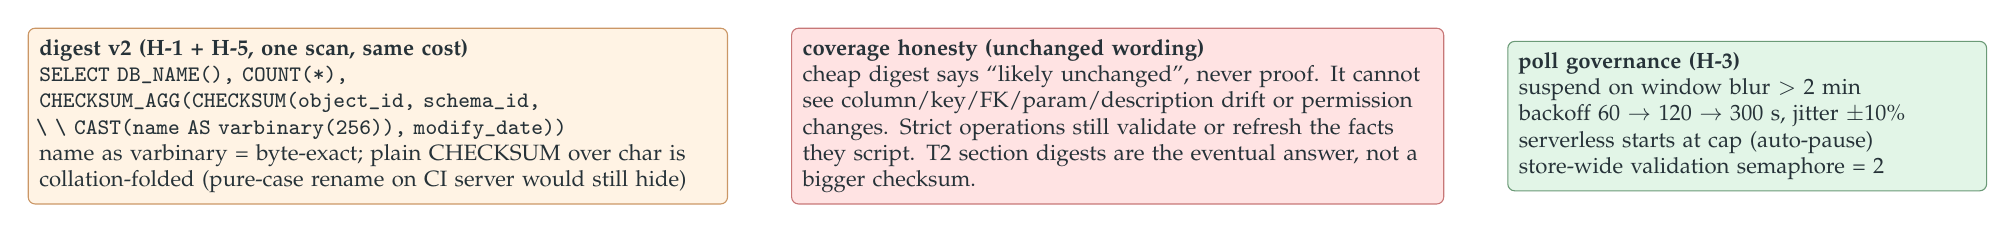
\begin{tikzpicture}[node distance=5mm and 8mm]
\node[enginebox,text width=86mm,align=left,font=\footnotesize] (v2) {\textbf{digest v2 (H-1 + H-5, one scan, same cost)}\\ \code{SELECT DB_NAME(), COUNT(*),}\\ \code{CHECKSUM_AGG(CHECKSUM(object_id, schema_id,}\\ \code{\ \ CAST(name AS varbinary(256)), modify_date))}\\ name as varbinary = byte-exact; plain CHECKSUM over char is collation-folded (pure-case rename on CI server would still hide)};
\node[riskbox,text width=80mm,right=8mm of v2,align=left,font=\footnotesize] (hon) {\textbf{coverage honesty (unchanged wording)}\\ cheap digest says ``likely unchanged'', never proof. It cannot see column/key/FK/param/description drift or permission changes. Strict operations still validate or refresh the facts they script. T2 section digests are the eventual answer, not a bigger checksum.};
\node[goodbox,text width=58mm,right=8mm of hon,align=left,font=\footnotesize] (pol) {\textbf{poll governance (H-3)}\\ suspend on window blur $>$ 2 min\\ backoff 60 $\to$ 120 $\to$ 300 s, jitter $\pm$10\%\\ serverless starts at cap (auto-pause)\\ store-wide validation semaphore = 2};
\end{tikzpicture}

\newpage

% =====================================================================
% A5. SEQUENCES: COLD START / STRICT SCRIPTING
% =====================================================================
\pagehead{A5. Two sequences: cold-start allowStale, and requireLive with a refusal leg}
{Left: the headline win - completion answers from disk in milliseconds while truth catches up. Right: strict scripting never silently downgrades.}
\legend\par\vspace{4mm}

\begin{adjustbox}{max width=\linewidth,max height=0.82\textheight,center}
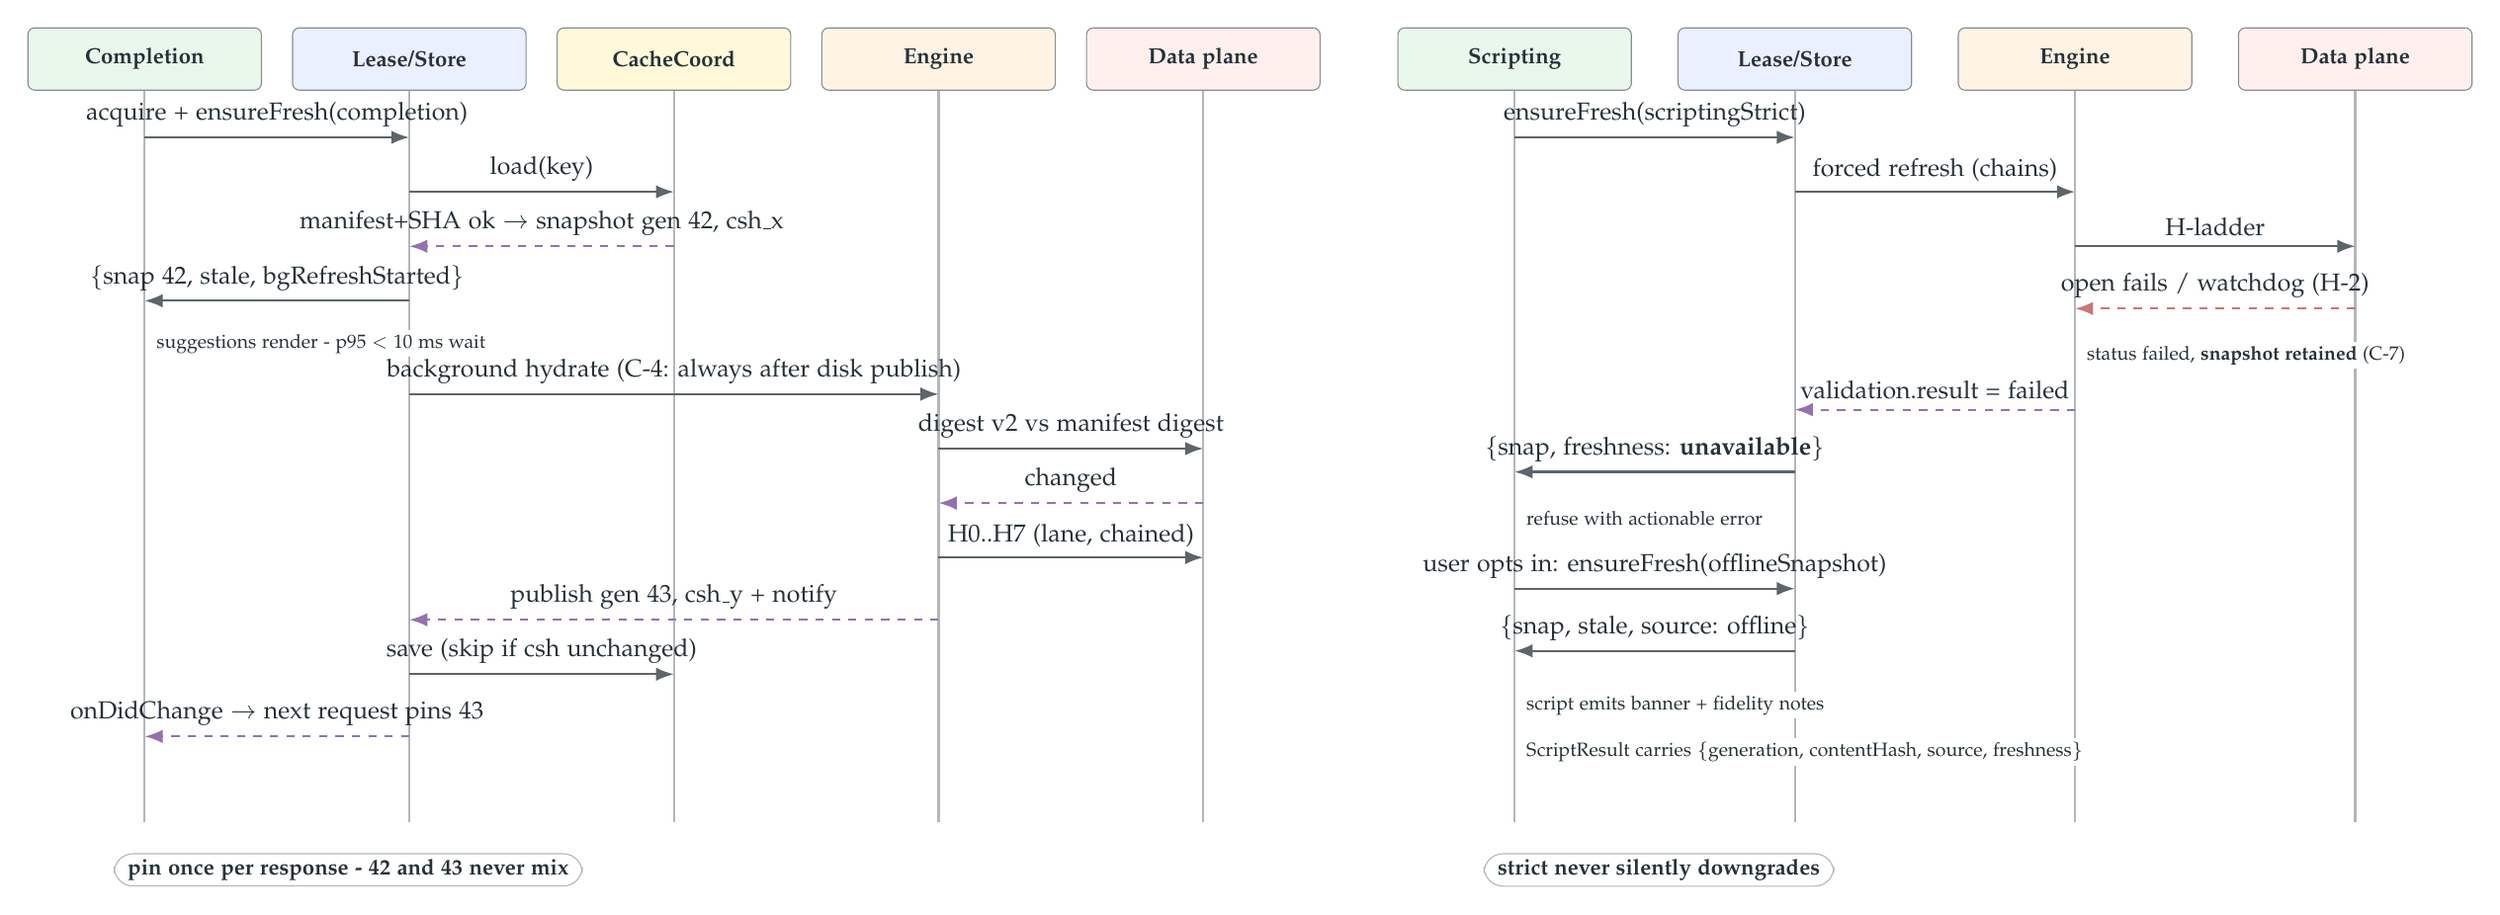
\begin{tikzpicture}[node distance=0mm]

% ---------- left sequence ----------
\node[head,fill=snap] (l1) at (0,0) {Completion};
\node[head] (l2) at (3.4,0) {Lease/Store};
\node[head,fill=future] (l3) at (6.8,0) {CacheCoord};
\node[head,fill=engine] (l4) at (10.2,0) {Engine};
\node[head,fill=session] (l5) at (13.6,0) {Data plane};
\foreach \n in {l1,l2,l3,l4,l5} {\draw[life] (\n.south) -- ++(0,-9.4);}

\draw[msg] ($(l1.south)+(0,-0.6)$) -- node[above]{acquire + ensureFresh(completion)} ($(l2.south)+(0,-0.6)$);
\draw[msg] ($(l2.south)+(0,-1.3)$) -- node[above]{load(key)} ($(l3.south)+(0,-1.3)$);
\draw[msgd] ($(l3.south)+(0,-2.0)$) -- node[above]{manifest+SHA ok $\to$ snapshot gen 42, csh\_x} ($(l2.south)+(0,-2.0)$);
\draw[msg] ($(l2.south)+(0,-2.7)$) -- node[above]{\{snap 42, stale, bgRefreshStarted\}} ($(l1.south)+(0,-2.7)$);
\node[caption,anchor=west] at ($(l1.south)+(0.1,-3.25)$) {\scriptsize suggestions render - p95 $<$ 10 ms wait};
\draw[msg] ($(l2.south)+(0,-3.9)$) -- node[above]{background hydrate (C-4: always after disk publish)} ($(l4.south)+(0,-3.9)$);
\draw[msg] ($(l4.south)+(0,-4.6)$) -- node[above]{digest v2 vs manifest digest} ($(l5.south)+(0,-4.6)$);
\draw[msgd] ($(l5.south)+(0,-5.3)$) -- node[above]{changed} ($(l4.south)+(0,-5.3)$);
\draw[msg] ($(l4.south)+(0,-6.0)$) -- node[above]{H0..H7 (lane, chained)} ($(l5.south)+(0,-6.0)$);
\draw[msgd] ($(l4.south)+(0,-6.8)$) -- node[above]{publish gen 43, csh\_y + notify} ($(l2.south)+(0,-6.8)$);
\draw[msg] ($(l2.south)+(0,-7.5)$) -- node[above]{save (skip if csh unchanged)} ($(l3.south)+(0,-7.5)$);
\draw[msgd] ($(l2.south)+(0,-8.3)$) -- node[above]{onDidChange $\to$ next request pins 43} ($(l1.south)+(0,-8.3)$);
\node[pill,anchor=north west] at ($(l1.south)+(-0.4,-9.8)$) {pin once per response - 42 and 43 never mix};

% ---------- right sequence ----------
\begin{scope}[xshift=176mm]
\node[head,fill=snap] (r1) at (0,0) {Scripting};
\node[head] (r2) at (3.6,0) {Lease/Store};
\node[head,fill=engine] (r3) at (7.2,0) {Engine};
\node[head,fill=session] (r4) at (10.8,0) {Data plane};
\foreach \n in {r1,r2,r3,r4} {\draw[life] (\n.south) -- ++(0,-9.4);}

\draw[msg] ($(r1.south)+(0,-0.6)$) -- node[above]{ensureFresh(scriptingStrict)} ($(r2.south)+(0,-0.6)$);
\draw[msg] ($(r2.south)+(0,-1.3)$) -- node[above]{forced refresh (chains)} ($(r3.south)+(0,-1.3)$);
\draw[msg] ($(r3.south)+(0,-2.0)$) -- node[above]{H-ladder} ($(r4.south)+(0,-2.0)$);
\draw[failarr] ($(r4.south)+(0,-2.8)$) -- node[above]{open fails / watchdog (H-2)} ($(r3.south)+(0,-2.8)$);
\node[caption,anchor=west] at ($(r3.south)+(0.1,-3.4)$) {\scriptsize status failed, \textbf{snapshot retained} (C-7)};
\draw[msgd] ($(r3.south)+(0,-4.1)$) -- node[above]{validation.result = failed} ($(r2.south)+(0,-4.1)$);
\draw[msg] ($(r2.south)+(0,-4.9)$) -- node[above]{\{snap, freshness: \textbf{unavailable}\}} ($(r1.south)+(0,-4.9)$);
\node[caption,anchor=west] at ($(r1.south)+(0.1,-5.5)$) {\scriptsize refuse with actionable error};
\draw[msg] ($(r1.south)+(0,-6.4)$) -- node[above]{user opts in: ensureFresh(offlineSnapshot)} ($(r2.south)+(0,-6.4)$);
\draw[msg] ($(r2.south)+(0,-7.2)$) -- node[above]{\{snap, stale, source: offline\}} ($(r1.south)+(0,-7.2)$);
\node[caption,anchor=west] at ($(r1.south)+(0.1,-7.9)$) {\scriptsize script emits banner + fidelity notes};
\node[caption,anchor=west] at ($(r1.south)+(0.1,-8.5)$) {\scriptsize ScriptResult carries \{generation, contentHash, source, freshness\}};
\node[pill,anchor=north west] at ($(r1.south)+(-0.4,-9.8)$) {strict never silently downgrades};
\end{scope}

\end{tikzpicture}
\end{adjustbox}

\newpage

% =====================================================================
% A6. SESSION LANE + STS2 INTERLOCKS
% =====================================================================
\pagehead{A6. The session lane under failure: watchdog, recycle, and the STS2 interlocks}
{The completion-reaction discipline assumes exactly one \code{v2/query.complete} per accepted execute. Until STS2-R008/R009/R010 land, the lane must be able to survive a completion that never comes.}
\legend\par\vspace{4mm}

\begin{adjustbox}{max width=\linewidth,max height=0.82\textheight,center}
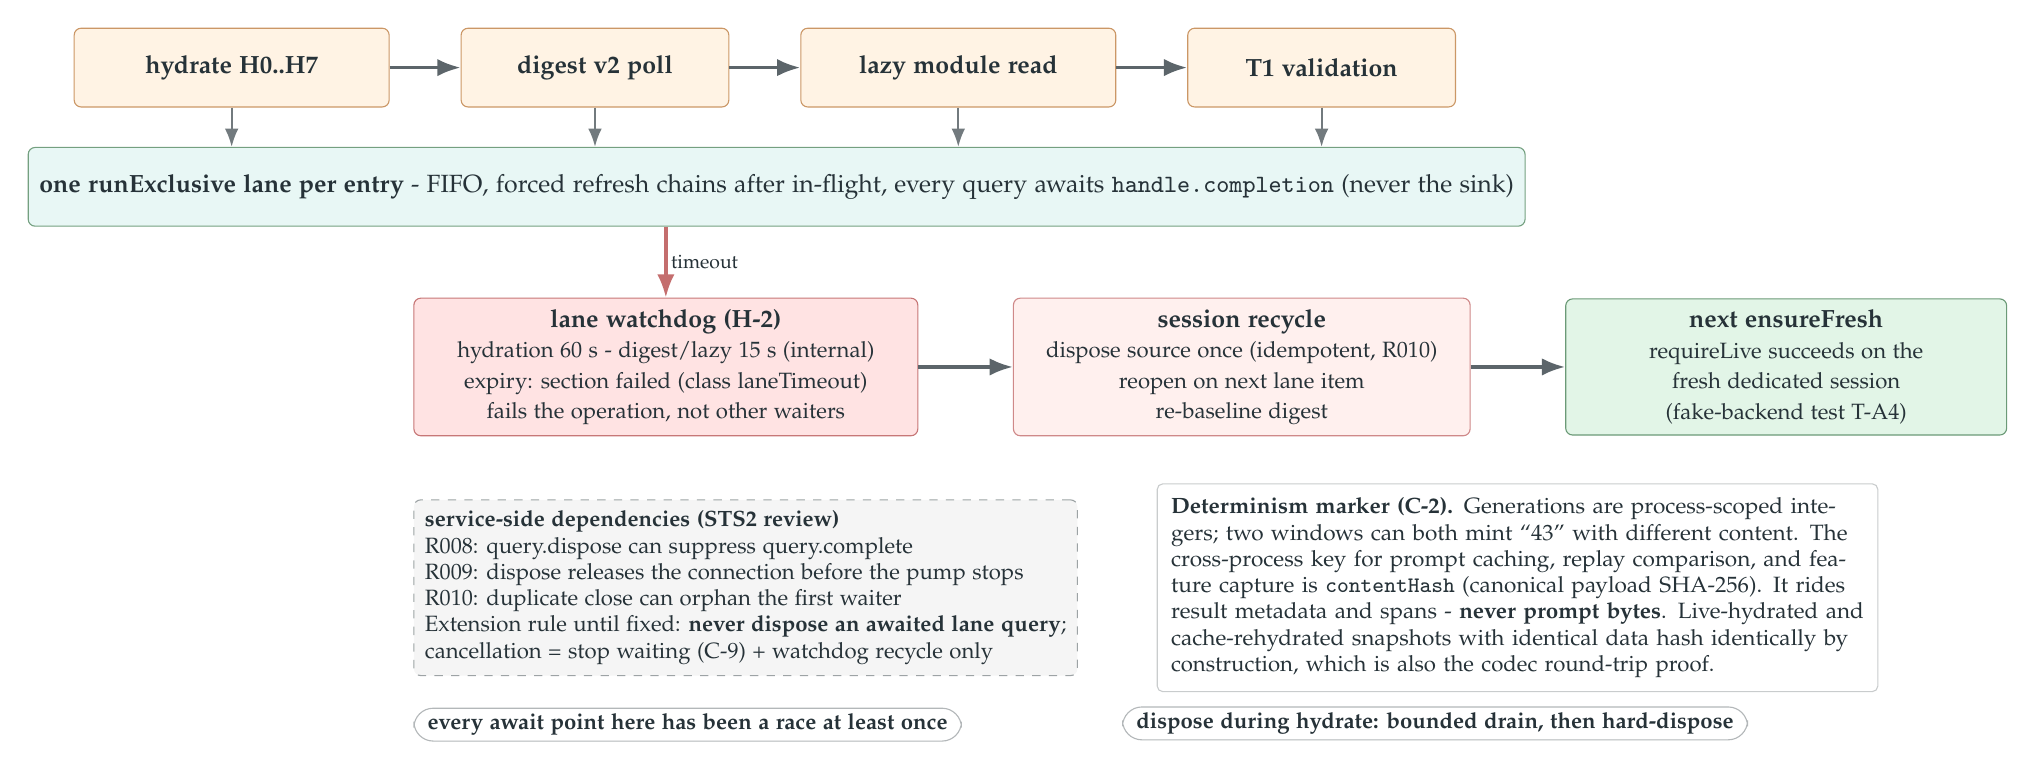
\begin{tikzpicture}[node distance=6mm and 9mm]

% lane
\node[enginebox,minimum width=40mm] (q1) {\textbf{hydrate H0..H7}};
\node[enginebox,minimum width=34mm,right=of q1] (q2) {\textbf{digest v2 poll}};
\node[enginebox,minimum width=40mm,right=of q2] (q3) {\textbf{lazy module read}};
\node[enginebox,minimum width=34mm,right=of q3] (q4) {\textbf{T1 validation}};
\draw[arrow] (q1) -- (q2);\draw[arrow] (q2) -- (q3);\draw[arrow] (q3) -- (q4);
\node[gatebox,minimum width=156mm,below=5mm of $(q2.south)!0.5!(q3.south)$] (lane) {\textbf{one runExclusive lane per entry} - FIFO, forced refresh chains after in-flight, every query awaits \code{handle.completion} (never the sink)};
\foreach \q in {q1,q2,q3,q4} {\draw[thinarr] (\q.south) -- (lane.north -| \q.south);}

% watchdog + recycle
\node[riskbox,minimum width=64mm,below left=9mm and -18mm of lane.south] (wd) {\textbf{lane watchdog (H-2)}\\\footnotesize hydration 60 s - digest/lazy 15 s (internal)\\\footnotesize expiry: section failed (class laneTimeout)\\\footnotesize fails the operation, not other waiters};
\node[sessbox,minimum width=58mm,right=12mm of wd] (rec) {\textbf{session recycle}\\\footnotesize dispose source once (idempotent, R010)\\\footnotesize reopen on next lane item\\\footnotesize re-baseline digest};
\node[goodbox,minimum width=56mm,right=12mm of rec] (next) {\textbf{next ensureFresh}\\\footnotesize requireLive succeeds on the\\\footnotesize fresh dedicated session\\\footnotesize (fake-backend test T-A4)};
\draw[hot] (lane.south -| wd.north) -- node[caption,right]{timeout} (wd.north);
\draw[arrow] (wd.east) -- (rec.west);
\draw[arrow] (rec.east) -- (next.west);

% STS2 findings
\node[extbox,minimum width=76mm,below=8mm of wd.south west,anchor=north west,align=left,font=\footnotesize] (sts) {\textbf{service-side dependencies (STS2 review)}\\
R008: query.dispose can suppress query.complete\\
R009: dispose releases the connection before the pump stops\\
R010: duplicate close can orphan the first waiter\\
Extension rule until fixed: \textbf{never dispose an awaited lane query};\\ cancellation = stop waiting (C-9) + watchdog recycle only};
\node[note,right=10mm of sts,text width=88mm,align=left] (det) {\textbf{Determinism marker (C-2).} Generations are process-scoped integers; two windows can both mint ``43'' with different content. The cross-process key for prompt caching, replay comparison, and feature capture is \code{contentHash} (canonical payload SHA-256). It rides result metadata and spans - \textbf{never prompt bytes}. Live-hydrated and cache-rehydrated snapshots with identical data hash identically by construction, which is also the codec round-trip proof.};

\node[pill,below=4mm of sts.south west,anchor=north west] {every await point here has been a race at least once};
\node[pill,right=6mm of {$(sts.south west)+(84mm,-6mm)$}] {dispose during hydrate: bounded drain, then hard-dispose};

\end{tikzpicture}
\end{adjustbox}

\end{document}
